\documentclass[a4paper,12pt, oneside]{book}
% \usepackage{fullpage}
\usepackage[italian]{babel}
\usepackage[utf8]{inputenc}
\usepackage{amssymb}
\usepackage{amsthm}
\usepackage{graphics}
\usepackage{amsfonts}
\usepackage{listings}
\usepackage{amsmath}
\usepackage{amstext}
\usepackage{bookmark}
\usepackage{engrec}
\usepackage{rotating}
\usepackage{verbatim}
\usepackage[safe,extra]{tipa}
%\usepackage{showkeys}
\usepackage{multirow}
\usepackage{hyperref}
\usepackage{epigraph}
\usepackage{microtype}
\usepackage{enumerate}
\usepackage{svg}
\usepackage{braket}
\usepackage{physics}
\usepackage{marginnote}
\usepackage{pgfplots}
\usepackage{lipsum}
\usepackage{cancel}
\usepackage{polynom}
\usepackage{booktabs}
\usepackage{enumitem}
\usepackage{framed}
\usepackage{pdfpages}
\usepackage{pgfplots}
\usepackage{algorithm}
\usepackage{graphicx}
% \usepackage{algpseudocode}
\usepackage{mathtools}
\usepackage[noend]{algpseudocode}
\usepackage{fancyhdr}
\usepackage{xpatch}
\usepackage{inputenc}
\usepackage{fontenc}
\usepackage{csquotes}
\usepackage[backend=biber, style=numeric, sorting=none, citestyle=reading]{biblatex}
\addbibresource{references.bib}

\setcounter{secnumdepth}{3}


\graphicspath{ {Immagini/} }
\setcounter{figure}{0}


\renewcommand\epigraphflush{flushright}
\renewcommand\epigraphsize{\normalsize}
\setlength\epigraphwidth{0.7\textwidth}

\renewcommand{\baselinestretch}{1.2}
\setlength{\parskip}{0.4em}

\usetikzlibrary{automata,positioning}
\setlength{\parindent}{0pt}

\pagestyle{plain}

\usepackage{tikz}
\usetikzlibrary{shapes.geometric, arrows}
\tikzstyle{startstop} = [rectangle, rounded corners, minimum width=3cm, minimum height=1cm,text centered, draw=black, fill=red!30]
\tikzstyle{io} = [trapezium, trapezium left angle=70, trapezium right angle=110, minimum width=3cm, minimum height=1cm, text centered, draw=black, fill=blue!30]
\tikzstyle{process} = [rectangle, minimum width=3cm, minimum height=1cm, text centered, draw=black, fill=orange!30]
\tikzstyle{decision} = [diamond, minimum width=3cm, minimum height=1cm, text centered, draw=black, fill=green!30]

% \usepackage{graphicx}
% \tikzstyle{arrow} = [thick,->,>=stealth]
% \setlist[itemize]{leftmargin=1em}
% \setlist[enumerate]{leftmargin=2em}

\definecolor{darkgreen}{rgb}{0.03,0.43, 0.30}
\usepackage[usenames,dvipsnames]{pstricks}
\usepackage{epsfig}
\usepackage{pst-grad} % For gradients
\usepackage{pst-plot} % For axes
\usepackage[space]{grffile} % For spaces in paths
\usepackage{etoolbox} % For spaces in paths
\makeatletter % For spaces in paths
\patchcmd\Gread@eps{\@inputcheck#1 }{\@inputcheck"#1"\relax}{}{}


\pgfplotsset{compat=1.13}
\definecolor{titlepagecolor}{cmyk}{1,1,0,0}

\DeclareFixedFont{\titlefont}{T1}{ppl}{b}{it}{0.5in}

\makeatletter                       
\def\printauthor{%                  
    {\large \@author}}              
\makeatother
\author{%
    Artemisia Sarteschi \quad 829677 \\
    Nicola Armas \quad 816398\\
    }

% The following code is borrowed from: https://tex.stackexchange.com/a/86310/10898

\newcommand\titlepagedecoration{%
\begin{tikzpicture}[remember picture,overlay,shorten >= -10pt]

\coordinate (aux1) at ([yshift=-15pt]current page.north east);
\coordinate (aux2) at ([yshift=-410pt]current page.north east);
\coordinate (aux3) at ([xshift=-4.5cm]current page.north east);
\coordinate (aux4) at ([yshift=-150pt]current page.north east);

\begin{scope}[titlepagecolor!40,line width=12pt,rounded corners=12pt]
\draw
  (aux1) -- coordinate (a)
  ++(225:5) --
  ++(-45:5.1) coordinate (b);
\draw[shorten <= -10pt]
  (aux3) --
  (a) --
  (aux1);
\draw[opacity=0.6,titlepagecolor,shorten <= -10pt]
  (b) --
  ++(225:2.2) --
  ++(-45:2.2);
\end{scope}
\draw[titlepagecolor,line width=8pt,rounded corners=8pt,shorten <= -10pt]
  (aux4) --
  ++(225:0.8) --
  ++(-45:0.8);
\begin{scope}[titlepagecolor!70,line width=6pt,rounded corners=8pt]
\draw[shorten <= -10pt]
  (aux2) --
  ++(225:3) coordinate[pos=0.45] (c) --
  ++(-45:3.1);
\draw
  (aux2) --
  (c) --
  ++(135:2.5) --
  ++(45:2.5) --
  ++(-45:2.5) coordinate[pos=0.3] (d);   
\draw 
  (d) -- +(45:1);
\end{scope}
\end{tikzpicture}%
}


% \pagestyle{fancy}
% \fancyhf{}
% \lhead{ \leftmark}
% \rhead{\rightmark}
% \rfoot{\thepage}

\begin{document}


\begin{titlepage}

\noindent
\titlefont Progetto \\ Sistemi Complessi: \\Modelli e Simulazione \par
\vspace*{3cm}

\epigraph{Progetto per il corso di  Sistemi Complessi: Modelli e Simulazione aa.2020/21 }
{}
\null\vfill
\vspace*{1cm}
\noindent
\hfill
\begin{minipage}{0.80\linewidth}
    \begin{flushright}
        \printauthor
    \end{flushright}
\end{minipage}
%
\begin{minipage}{0.02\linewidth}
    \rule{1pt}{125pt}
\end{minipage}
\titlepagedecoration
\end{titlepage}

%\maketitle
%\definecolor{shadecolor}{gray}{0.90}
%\setlist{leftmargin = 2cm}
%\newcommand{\normm}[1]{\left\lVert#1\right\rVert}


\tableofcontents
\chapter{Introduzione}

Il tema di questo progetto è basato sostanzialmente sullo studio esplorativo del software AnyLogic, utilizzando un problema del mondo reale come quello di ottimizzazione delle tempistiche di un pronto soccorso.

Siamo quindi andati valutare come questo strumento si comportasse nel modellare questa situazione per valutarne le funzionalità utilizzando un approccio ad agenti. 
All’interno di un pronto soccorso gravitano diverse figure e i pazienti possono arrivare in condizioni molto diverse.

Abbiamo scelto di utilizzare AnyLogic per conoscere un software differente da quelli proposti nel corso e capire se, essendo fornito ed utilizzato a livello commerciale, potesse fornire degli strumenti migliori per rendersi potenzialmente comprensibile ad un gruppo di persone interessate all’argomento ma non ferrate sulla simulazione.

Nei prossimi capitoli di questo documento descriveremo il software scelto, con un approfondimento sul modello ad agenti realizzato e simulato grazie ad esso; infine, analizzeremo i risultati ottenuti da alcune sperimentazioni eseguite, al fine di confrontarli con quello che è lo stato dell'arte attuale, ovvero gli articoli su cui ci siamo basati per fondare il nostro modello. 

All'interno del \href{https://github.com/NArmas-unimib/SC-EmergencyRoom/tree/main}{repository} è possibile scaricare il file della simulazione in AnyLogic e visualizzare i video che ne mostrano il funzionamento.
\chapter{Stato dell'Arte}

In un contesto complesso, dinamico e spesso riservato come quello di un pronto soccorso, può risultare molto arduo ottenere informazioni volte a realizzarne una rappresentazione, seppur in forma modellare, che si avvicini il più possibile al sistema reale. 
 
Per questo motivo è spesso utile per un modellista basarsi su quello che è chiamato lo \textit{``stato dell'arte"}: articoli scientifici, libri e strumenti che descrivono il massimo livello di sviluppo nella ricerca in un determinato ambito. 

Nel caso in esame, abbiamo deciso di basarci sul lavoro di diversi ricercatori che avessero già approfondito il tema, tramite progetti riportati sotto forma di paper scientifici.  

\section{Paper}

Gli articoli scientifici su cui si è basato il nostro modello sono i seguenti:
\begin{itemize}
\item \cite{garcia_reducing_1995}
\item \cite{espinoza_real-time_2014}
\item \cite{stainsby_towards_2009} 
\item  \cite{wang_agent-based_2009}
\end{itemize}


Il lavoro svolto in ciascuna di queste ricerche è servito principalmente a non dover sviluppare un nuovo modello partendo da zero: è risultato infatti difficile ottenere informazioni direttamente sul campo, a causa della riservatezza caratteristica dell'ambiente in oggetto. 

In particolare, i paper \textit{\cite{garcia_reducing_1995}}, \textit{\cite{stainsby_towards_2009}} e \textit{\cite{wang_agent-based_2009}} sono risultati utili a definire un workflow (vedi \textit{Capitolo 4}) che potesse dare forma all'interazione degli agenti con l'ambiente, ai percorsi seguiti e alle risorse utilizzate.

\begin{figure}[!htb]
    \centering
    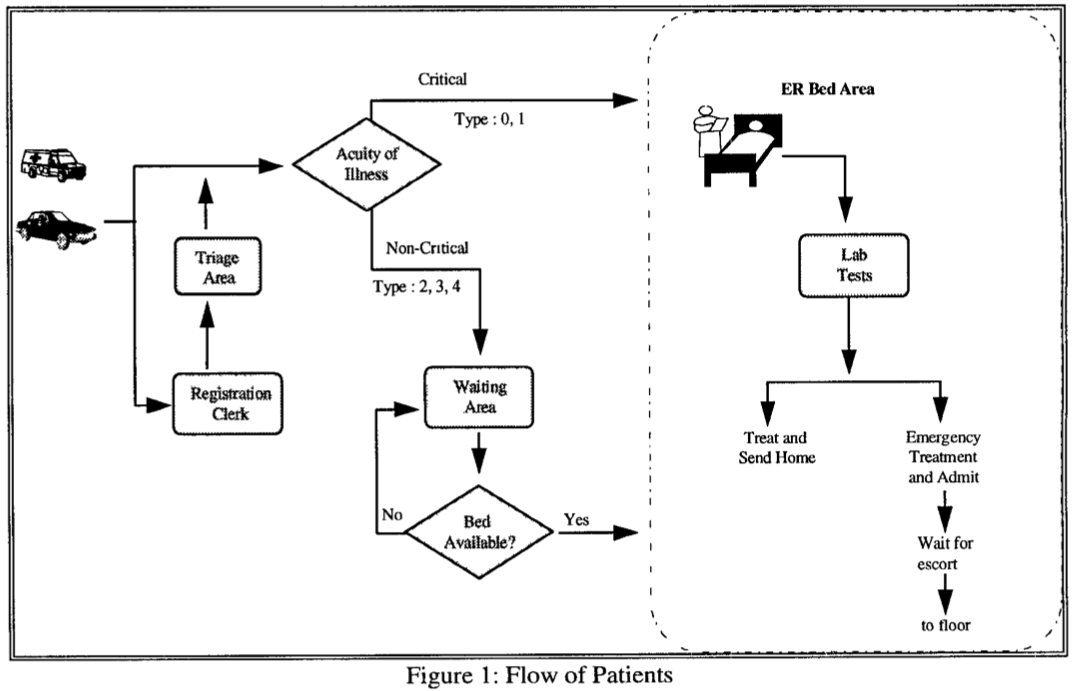
\includegraphics[width=1\textwidth]{Immagini/garcia-wf.png} 
    \caption{Workflow utilizzato nel paper \textit{\cite{garcia_reducing_1995}}}
\end{figure}

\begin{figure}[!htb]
    \centering
    \makebox[\textwidth][c]{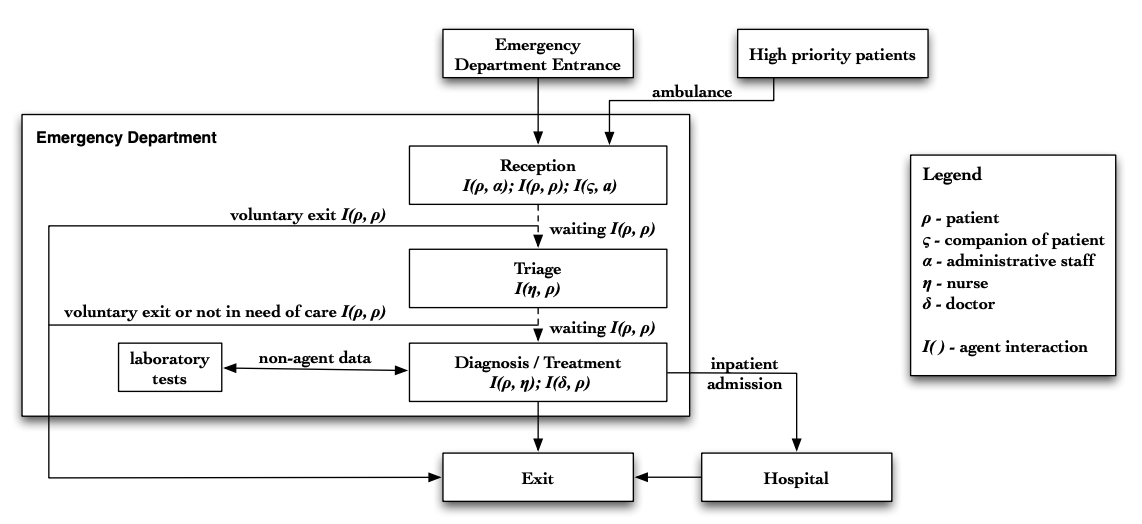
\includegraphics[width=1\textwidth]{Immagini/stainsby-wf.png}}   
    \caption{Workflow utilizzato nel paper \textit{\cite{stainsby_towards_2009}}}
\end{figure}

\begin{figure}[!htb]
    \centering
    \makebox[\textwidth][c]{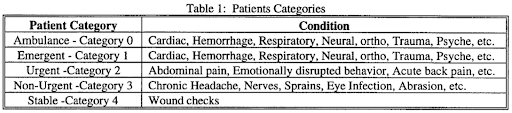
\includegraphics[width=1\textwidth]{Immagini/garcia-priority.png}}   
    \caption{Codici di priorità utilizzati nel paper \textit{\cite{stainsby_towards_2009}}}
\end{figure}

\begin{figure}[!htb]
    \centering
    \makebox[\textwidth][c]{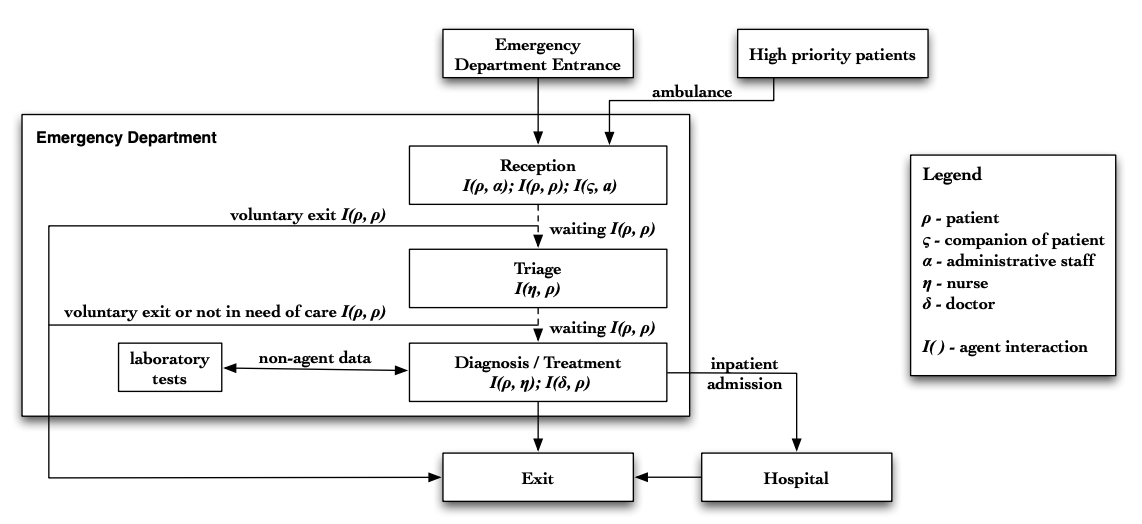
\includegraphics[width=1\textwidth]{Immagini/stainsby-wf.png}}   
    \caption{Codici di priorità reperibili dal sito della \textit{Regione Lombardia}}
\end{figure}

Il paper \textit{\cite{espinoza_real-time_2014}} è servito a definire delle metriche per effettuare sperimentazioni e a confrontarne i risultati con quelli ottenuti nei lavori precedenti (vedi \textit{Capitolo 5}). 

Infine, consultando nuovamente il paper \textit{\cite{garcia_reducing_1995}} e confrontandolo con le informazioni riportate sul sito della \textit{Regione Lombardia} (per un maggiore adattamento a quello che è il modello locale), è risultato possibile ottenere una rappresentazione tabellare della gravità tipica dei pazienti ed annessa priorità. 


\clearpage
\section{Strumenti}

Per completare l'approfondimento relativo a quello che è lo stato dell'arte, in questa sezione verranno descritti brevemente gli strumenti utilizzati in ciascuno dei paper consultati. 

È doveroso riportare che solo in uno di questi lavori non è stata effettuata una simulazione né sono stati adoperati strumenti informatici di supporto: in particolare, nel paper \textit{\cite{stainsby_towards_2009}} è stato realizzato unicamente il modello matematico per il raggiungimento di un modello ad agenti simulabile (il titolo recita ``\textit{towards}", per l'appunto).

\subsection{Garcia et al., 1995: \textit{SIMAN}}

Lo strumento utilizzato in questo paper per simulare il modello è un linguaggio chiamato SIMAN (SIMulation ANalysis), presentato nel 1982 nell'articolo \textit{\cite{pegden_simulation_1982}}. 

È utilizzato per modellare sistemi combinati discreto-continui, tramite l'impiego di diversi approcci: per il discreto, si orienta verso l'utilizzo di \textit{processi} oppure \textit{eventi}. 
La parte continua è modellata tramite \textit{algebra, differenze} o \textit{equazioni differenziali}. 


\subsection{Espinoza et al., 2014: \textit{FlexSim HC}}

FlexSim HC (HealthCare) è un ambiente di simulazione sviluppato da FlexSim, adoperato  a livello aziendale nell'ambito della salute. 
In maniera simile ad AnyLogic, permette di modellare un ambiente 3D ed un workflow per orientare pazienti e staff all'interno del detto ambiente. 

Sul \underline{\href{https://www.flexsim.com/healthcare/flexsim-hc/}{sito Internet dedicato}} è possibile scaricarne una versione di prova gratuita per testarne le funzionalità. 

\subsection{Wang, 2009: \textit{NetLogo}}

NetLogo è un linguaggio di programmazione e IDE per la modellazione basata su agenti. 
Presentato nel 1999, è particolarmente efficace per l'esplorazione di \textit{fenomeni emergenti}, di cui include una vasta libreria di modelli al suo interno. 

NetLogo è open-source e scaricabile gratuitamente dal \underline{\href{http://ccl.northwestern.edu/netlogo/}{suo sito Internet}}. 






\chapter{AnyLogic}
AnyLogic è uno strumento per creare modelli di simulazione sviluppato da The AnyLogic Company.
Viene utilizzato nel contesto industriale in molti ambiti, come ad esempio: 
\begin{itemize}
    \item Healthcare
    \item Manifattura
    \item Pedoni e traffico
    \item Trasporti
    \item Catene di montaggio
\end{itemize}


Questo software include un linguaggio di modellazione grafico che si interfaccia con il linguaggio Java, offrendo all’utente svariate opzioni di personalizzazione e impostazione. 

L'utilizzo di AnyLogic per questo progetto è stato considerato e successivamente messo in atto per diversi motivi: primo fra tutti, la varietà degli ambiti di utilizzo possibili, molto elevata e adatta al caso in esame. \\
Un altro motivo importante è la possibilità di simulare modelli in ambienti anche tridimensionali, che rende questo software user-friendly anche per neofiti, obiettivo raggiunto grazie anche alla simulazione a blocchi, che permette una rappresentazione dei modelli chiara e funzionale. 
\\ In ultimo, oltre ai vantaggi sopra elencati, la possibilità di ottenere analisi statistiche in tempo reale su vaste popolazioni di agenti e la facoltà di potersi interfacciare con molti sistemi di gestione dati esterni hanno fatto ricadere la scelta su questo potente strumento. 


\section{Edizioni di AnyLogic e scelta della nostra}
AnyLogic offre una versione di prova, per un periodo di 30 giorni, delle sue versioni non gratuite (Professional e University Researcher). 

La scelta di usare la versione di prova dell’edizione Professional per questo progetto è dettata dalle limitazioni della versione gratuita PLE (Personal Learning Edition), in particolare la limitazione del tempo di simulazione a 60 minuti. 
Nonostante si sia deciso di utilizzare un’edizione Professional, tuttavia, la sua versione di prova presenta a sua volta delle grosse limitazioni: un esempio è quello di avere un limite massimo di 35 blocchi per workflow. 
Per il presente progetto, ciò è particolarmente arginante poiché lo scopo è quello di simulare un ambiente con molte interazioni e spostamenti. 

Alcuni possibili espedienti per risolvere questo problema possono essere: la divisione degli ambienti in più sotto-ambienti (progetti AnyLogic complementari), l'utilizzo della versione PLE con scala adatta delle tempistiche oppure, più drasticamente, l'acquisto della versione Professional completa.

\begin{figure}[!h]
    \centering
    \makebox[\textwidth][c]{
\includegraphics[width=1\textwidth]{Immagini/typeAnyLogic.png}}   
    \caption{Versioni di AnyLogic}
    \label{fig:window}
\end{figure}


\section{Piattaforma Cloud}
La piattaforma Cloud viene principalmente utilizzata per condividere i modelli realizzati con altri utenti oppure, in caso di contesti aziendali, con i propri clienti e dipendenti. 
Permette inoltre di integrare dati operazionali e di creare dashboard altamente personalizzabili in base al contesto (analisi, sperimentazione, gestione, ...). \\
Una caratteristica molto utile è quella di poter effettuare simulazioni distribuite: si possono partizionare modelli pesanti a livello di risorse in modelli più piccoli e, tramite l’utilizzo di API (JS, Java, Python), agevolare lo scambio di dati e la sincronizzazione tra essi per un’esecuzione più veloce. 
AnyLogic Cloud è offerto in due soluzioni: Public Cloud e Private Cloud. 

Mentre la prima è online, gratuita e disponibile a chiunque per il caricamento e la condivisione di modelli, la seconda opzione è un’infrastruttura vera e propria per organizzazioni e aziende, che viene installata in-house presso un data center o provider PaaS. Ciò permette di avere un controllo completo su dati e operazioni, integrando l’offerta di AnyLogic direttamente all’interno della propria azienda. 



\begin{figure}[!h]
    \centering
    \makebox[\textwidth][c]{
\includegraphics[width=\textwidth]{Immagini/cloud.png}}   
    \caption{Versioni del Cloud}
    \label{fig:window}
\end{figure}

\clearpage
\section{AI e ML}

AnyLogic fornisce un ambiente altamente strutturato per sviluppare simulazioni di ambienti reali con differenti approcci \textit{(system dynamics},  \textit{discrete event simulation} e\textit{ agent based}). 
\\ In riferimento all'ultimo approccio citato, ovvero \textit{agent based}, la piattaforma fornisce la possibilità di creare e progettare agenti capaci di imparare dalla loro esperienza: in particolare possono essere modellati l'intera gamma di agenti con comportamento cooperativo, competitivo o gerarchico. 
Abbiamo quindi la possibilità di impiegare la piattaforma per addestrare l'ambiente impiegato negli schemi di reinforcement learning multi agente.
Inoltre, AnyLogic Company mette a disposizione una piattaforma Cloud che può fornire una esecuzione parallela del modello, una facilità di condivisione e una RESTful API. 
AnyLogic appoggiandosi e/o collaborando con altre aziende fornisce al cliente tre possibilità per inserire l'intelligenza artificiale e più in generale varie forme di machine learning all'interno dei loro progetti.


\subsection{Project Bonsai}

Project Bonsai è un progetto nato dalla collaborazione tra The AnyLogic Company e Microsoft. L'obbiettivo di Bonsai è permettere agli esperti di dominio, anche privi di una conoscenza pregressa di \textit{Intelligenza Artificiale} (AI) di incorporare la loro esperienza attraverso il \textit{Machine Teaching} (MT) direttamente nei modelli e con l'aiuto della potenza del\textit{ Deep Reinforcement Learning }(DRL) ottimizzare e automatizzare i sistemi reali.\\
La collaborazione tra le due aziende si realizza con un connettore che permette di utilizzare i modelli sviluppati in AnyLogic come simulatori della piattaforma Bonsai. Ovvero per semplificare la conversione di questi modelli di simulazione (AnyLogic) in simulatori (Bonsai) è stato creato “RLExperiment” che permette di  esportare un modello con tutti i meccanismi integrati necessari per comunicare senza problemi con la piattaforma Project Bonsai.
\\ Nel caso in cui volessimo utilizzare questo strumento i passi sono i seguenti e nel caso si volesse un esempio di approfondimento lo si può trovare al seguente \href{https://microsoft.github.io/moab/tutorials/1-balance/index.html}{link}.

\subsubsection{Creare un Brain}
\begin{enumerate}
\item  Creare un account o collegarsi \href{https://preview.bons.ai/accounts/signin}{Bonsai}
\item  Cliccare su \texttt{Create brain} selezionare \texttt{Empty brain}.
\item  Nominarlo con un nome a scelta.
\end{enumerate}
A questo punto visualizziamo la schermata in figura \ref{fig:window}: se già possediamo un file \texttt{.ink} possiamo inserirlo all'interno della finestra \texttt{Teach} oppure scrivere in linguaggio proprietario \textit{Inkling} il codice per il MT, questo codice verrà anche chiamato \textit{curriculum}. 

Nella parte destra della schermata (\textit{Graphing panel}) è possibile avere anche una rappresentazione grafica interattiva del processo di apprendimento iterativo definito dal codice Inkling.


\begin{figure}[!h]
    \centering
    \makebox[\textwidth][c]{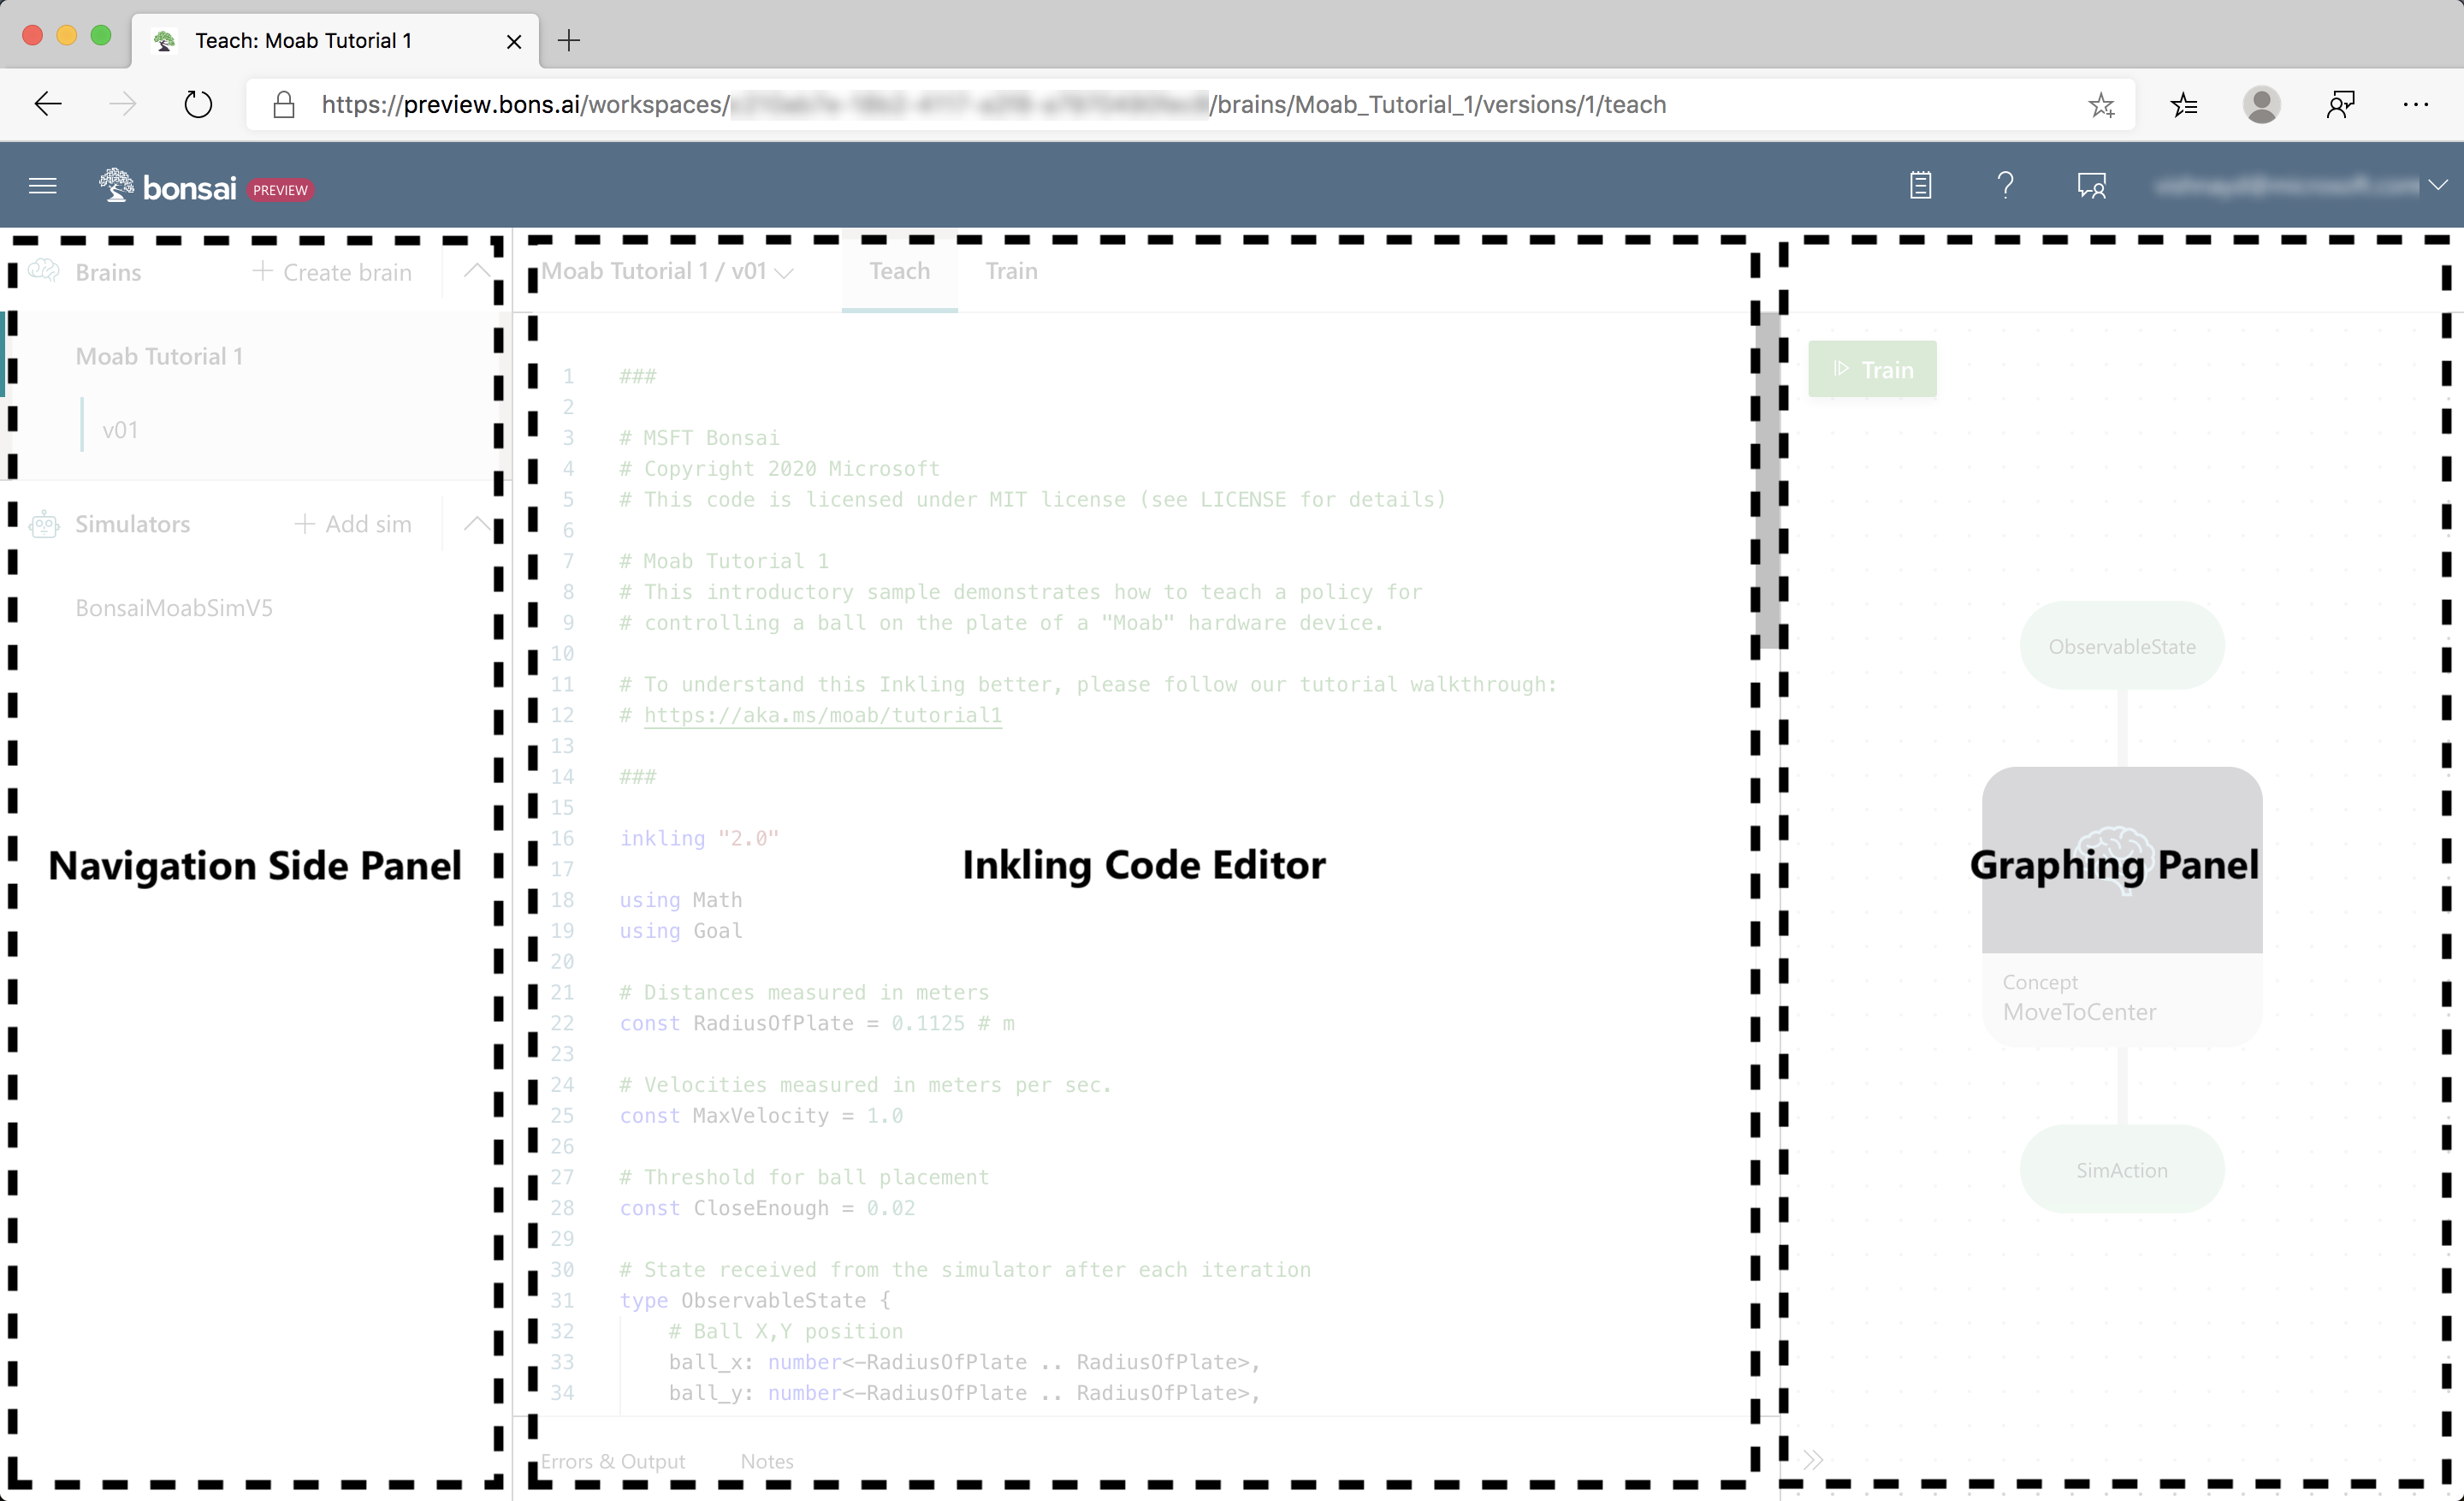
\includegraphics[width=1\textwidth]{Immagini/UI.png}}   
    \caption{Interfaccia di Bonsai}
    \label{fig:window}
\end{figure}

\subsubsection{Esecuzione del Modello}
A questo punto per eseguire il modello si può scegliere di farlo con un animazione: click destro su \texttt{AnimatedExperiment}, poi \texttt{Run} e dopo si visualizzerà in console la riuscita della registrazione alla piattaforma Bonsai tornare nella schermata dove è stato creato il brain. 
A questo punto si fa partire l'effettivo \texttt{train} del modello (azione diretta nel caso si sia scelto di eseguire un esperimento non animato), si vedrà quindi comparire un simulatore con il nome corrispondente su cui bisognerà cliccare.
\\ Nel caso fosse la prima volta che il brain viene eseguito potrebbero essere necessari diversi minuti per generare i parametri adatti e connettersi al simulatore. Si può far addestrare il brain per un lasso di tempo variabile, ma viene consigliato di tenere le iterazioni sotto le 1000, quando si ritiene siano sufficienti si cliccherà su \texttt{Stop Training}.

\subsubsection{Esportare e scalare il modello di Anylogic}
Il modello creato in AnyLogic necessita di essere esportato e compresso (\texttt{.zip}) per poter essere caricato su Bonsai. \\ Nel caso in cui si utilizzi \textit{AnyLogic Professional} sarà sufficiente selezionare nella barra dei menù \texttt{File > Export...> standalone Java application}, se si incontrassero delle difficoltà è disponibile il \href{https://anylogic.help}{supporto di Anylogic}.

Dopo questo passaggio è necessario importare il modello di Anylogic all'interno di Bonsai e per farlo sarà sufficiente selezionare su \texttt{Add sim} sull'interfaccia di Bonsai.
Si aprirà quindi la finestra di dialogo in figura \ref{fig:dialog} dove sarà sufficiente cliccare su AnyLogic, caricare il file \texttt{.zip} precedentemente creato e selezionare \texttt{Create simulator}. Il simulatore appena creato verrà visualizzato nella sezione \texttt{Simulators}.

\begin{figure}[!h]
    \centering
    \makebox[\textwidth][c]{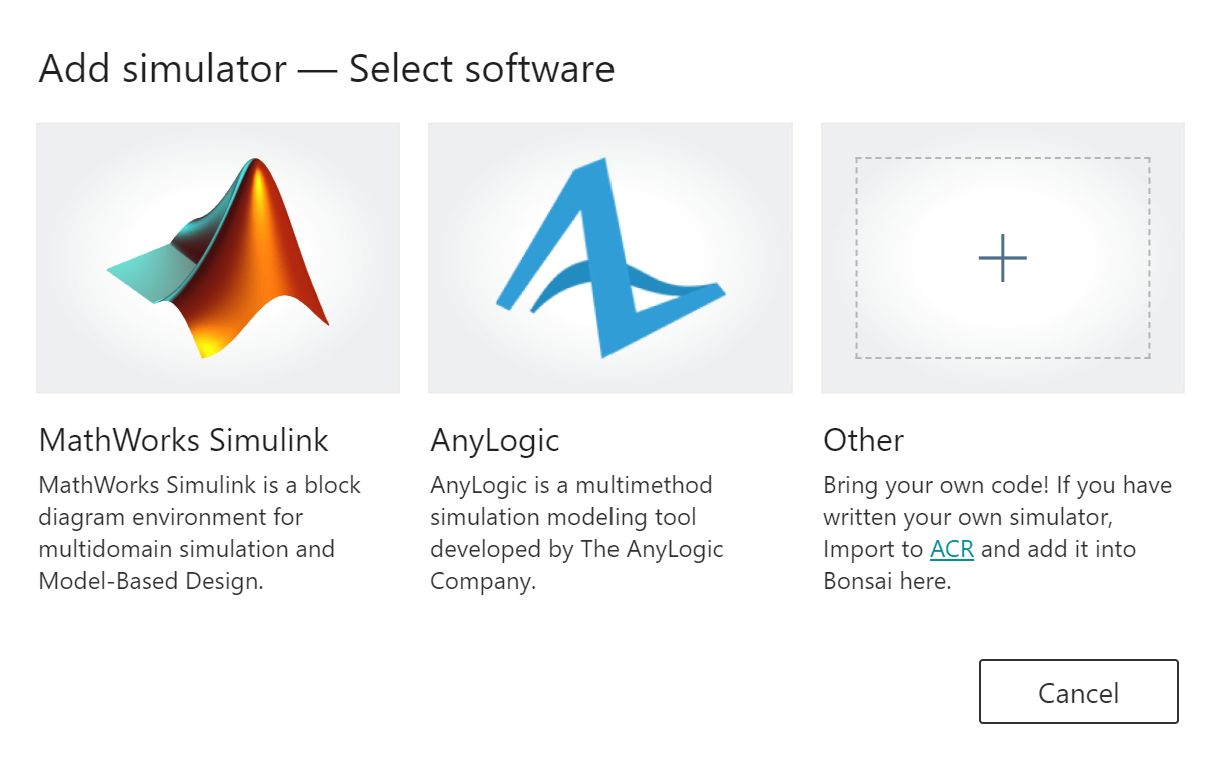
\includegraphics[width=1\textwidth]{Immagini/add_sim.png}}   
    \caption{Finestra per la scelta del simulatore}
    \label{fig:dialog}
\end{figure}
\clearpage
All'interno della scheda \texttt{Teach}, nella definizione del modello, è necessario aggiungere le seguenti linee di codice:

\begin{figure}[!h]
    \centering
    \makebox[\textwidth][c]{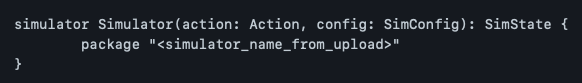
\includegraphics[width=1\textwidth]{Immagini/code.png}}   
    \label{fig:dialog}
\end{figure}

Si potrà quindi selezionare \texttt{Train} e dopo alcuni minuti si potranno vedere diversi simulatori collegati che addestrano il Brain. 

%----------------------------------------------------------------------

\subsection{H20.ai}
AnyLogic è partner di H2O.ai, una delle principali piattaforme di automatic machine learning. 
L’AutoML è una branca del ML che permette di applicare le tecniche di Ml ai problemi del mondo reale usando l’automazione. In particolare, automatizza la selezione, la composizione e la parametrizzazione dei modelli di machine learning.
L'obiettivo di integrare questi due sistemi è fornire la possibilità ai data scientist di testare le loro soluzioni in uno spazio sicuro e ai modellatori di accedere a una maggior quantità di input data-driven.

Le informazione per come utilizzare questa piattaforma con AnyLogic non sono accessibili al pubblico ma solo mettendosi in contatto con l'azienda. 
Le indicazioni che si possono ricavare dal \href{https://www.anylogic.com/features/artificial-intelligence/h2o-ai/}{sito di Anylogic} è la possibilità di scaricare da \textit{H2O.ai }il modello già addestrato per inserirlo all'interno delle simulazioni di AnyLogic ed utilizzarlo come fosse una funzione in grado di restituire delle predizioni basate sugl'input che vengono passati dinamicamente alla simulazione durante l'esecuzione.

%----------------------------------------------------------------------
\clearpage
\subsection{Pathmind}
La terza possibilità per inserire degli elementi di AI in AnyLogic è \textit{Pathmind}.
\\ Pathmind è una piattaforma SaaS che permette di avere accesso a delle tecniche di deep reinforcement learning e cloud computation per applicarle a degli scenari del mondo reale senza la necessità di avere esperienza di data science.

Pathmind a differenza dei servizi precedentemente presentati si va ad inserire all'interno di AnyLogic con Pathmind Helper attraverso cui è possibile agire sul modello.

Il processo da seguire per utilizzare Pathmind è il seguente: \begin{enumerate}
\item Creare un modello in AnyLogic che simuli un problema del mondo reale.
\item Usare Pathmind Helper per aggiungere il reinforcement learning all'interno della simulazione di AnyLogic.
\item Caricare la simulazione di AnyLogic in Pathmind, nel cui cloud avviene l'addestramento.
\item Scaricare i risultati ottenuti e validarli in AnyLogic.
\end{enumerate}

E' possibile trovare informazioni aggiuntive su Pathmind nel \href{https://help.pathmind.com/en/collections/2106204-tutorials-example-simulation-models#getting-started}{help} mantenuto dall'azienda. 

\clearpage
\subsubsection{Pathmind Helper}
All'interno di ogni agente che vogliamo dotare di AI abbiamo bisogno di creare un diagramma di stato e inserire Pathmind Helper come nell'esempio in figura \ref{fig:AIagent}. 

\begin{figure}[!h]
    \centering
    \makebox[\textwidth][c]{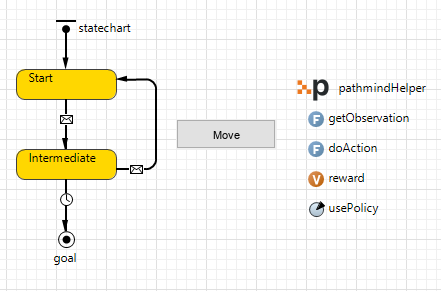
\includegraphics[width=200px]{Immagini/aiagent.png}}   
    \caption{Agente tipo}
    \label{fig:AIagent}
\end{figure}

Aprendo Pathmind Helper possiamo controllare i seguenti elementi del RL:
\begin{itemize}
\item \textbf{Number of Agents}: il numero di agenti "controllati" presenti nel modello.
\item \textbf{Observations}: contengono tutte le informazioni sullo stato corrente dell'ambiente.
\item \textbf{Metrics}: sono le metriche che vengono utilizzate all'interno della funzione di \textit{reward} per determinare se un'azione è stata buona o cattiva, a volte contiene anche il costo di essa. 
\item \textbf{Actions}: definisce tutte le azioni che un agente può svolgere.
\item \textbf{Done}: dal momento che tutte le simulazioni hanno necessità di un punto di arrivo, questo viene settato o dopo un lasso di tempo prestabilito o al raggiungimento di una determinata condizione.
\item \textbf{Event Trigger}: indicano a Pathmind quando inizia l'azione successiva, dopo un lasso di tempo o al verificarsi di una determinata condizione. 
\end{itemize}




All'interno di Pathmind Helper è possibile testare il modello, prima di esportarlo, spuntando la \texttt{Debug Mode} che permetterà di aprire il \texttt{Developer Panel} al cui interno, 
in caso in cui fosse tutto impostato correttamente, verrà stampata a video ogni azione che l'agente performa (figura \ref{fig:debugfig}).

\begin{figure}[!h]
    \centering
    \makebox[\textwidth][c]{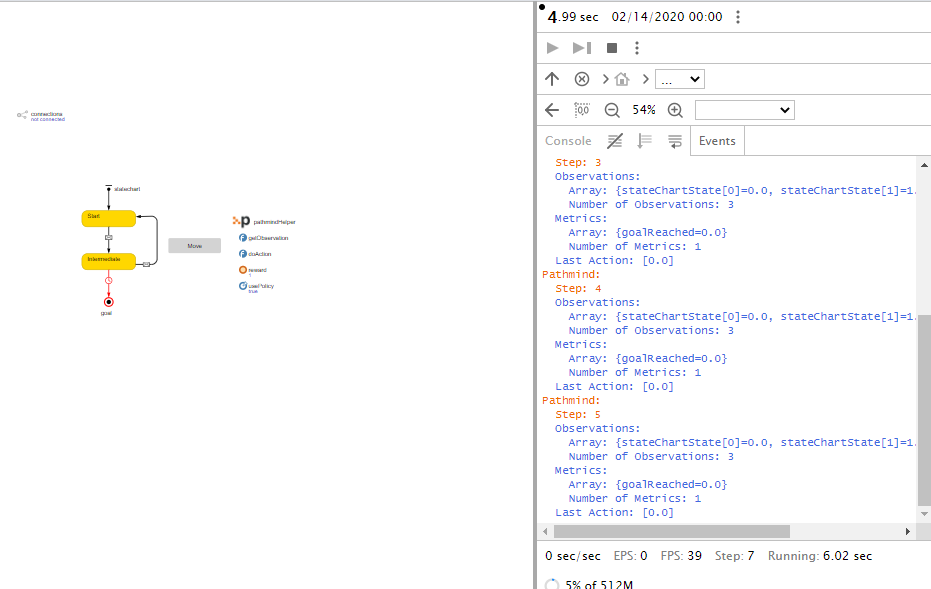
\includegraphics[width=1\textwidth]{Immagini/debug.png}}   
    \caption{Agente tipo}
    \label{fig:debugfig}
\end{figure}

Dopo che il modello è stato configurato è possibile esportarlo nell'applicazione web di Pathmind per l'addestramento. All'interno di questa web app è possibile configurare la funzione di reward ed addestrare con essa il modello in circa 10 minuti. 

Al termine dell'addestramento è possibile esportare la policy risultante e inserirla in Anylogic all'interno del Pathmind helper sotto \texttt{Policy File}. Seguendo la policy inserita l'agente convergerà all'obbiettivo nel minor numero di passi possibile.








\chapter{Modello}

\section{Ambiente costruito}

Prima di andare a definire gli agenti che operano nel nostro modello, abbiamo raccolto informazioni sulla possibile struttura dell'ambiente di un pronto soccorso, al fine di costruire una piantina che avesse le caratteristiche generiche di un pronto soccorso comune. 

In particolare, le stanze che abbiamo infine deciso di realizzare sono le seguenti: 
\begin{itemize}
    \item Sala d'attesa
    \item Accettazione: 2 file
    \item Triage: 2 stanze
    \item Sala visita: 4 stanze
    \item Chirurgia: 2 sale operatorie
    \item Degenza breve: 1 con posti letto normali, 1 con posti letto di emergenza
\end{itemize}

\begin{figure}[!htb]
    \centering
    \makebox[\textwidth][c]{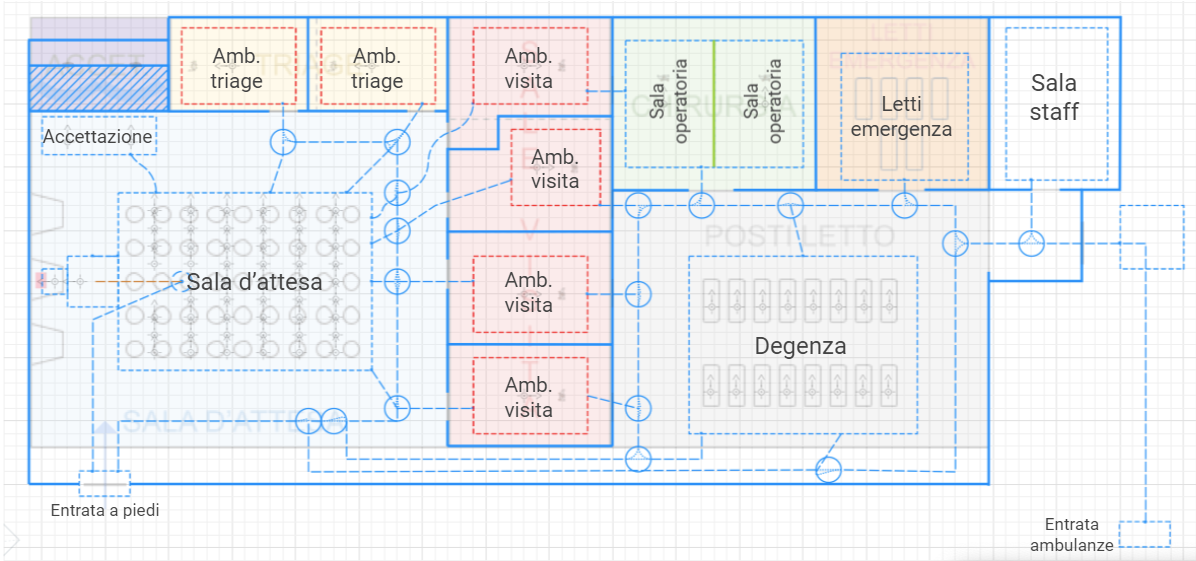
\includegraphics[width=1\textwidth]{layout}}   
    \caption{Layout 2D dell'ambiente costruito}
    \label{fig:layout}
\end{figure}
\begin{figure}[!htb]
    \centering
    \makebox[\textwidth][c]{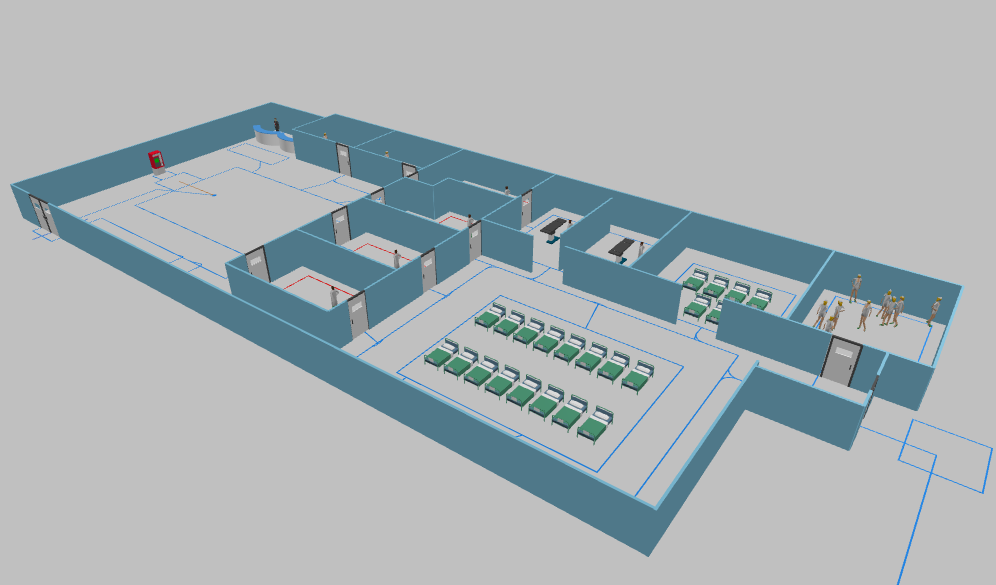
\includegraphics[width=1\textwidth]{3d presentation}}   
    \caption{Layout 3D dell'ambiente costruito}
    \label{fig:layout3D}
\end{figure}

\section{Agenti realizzati}

Gli agenti che abbiamo realizzato per impostare il funzionamento del modello sono Patient, Ambulance, AmbulancePatient e Nurse. 
Mentre i primi tre sono generati in base ad uno specifico tasso di input, gli infermieri appartengono ad una pool di risorse per cui vengono effettuate delle richieste all'occorrenza.

\subsection{Patient}

Questo agente è il più importante del modello: rappresenta infatti il paziente che si reca al pronto soccorso. E' caratterizzato da alcuni parametri che ne definiscono il comportamento all'interno del workflow: 

\paragraph{\textit{appearance}}
Definisce l'agente a livello puramente estetico tramite un'estrazione da una distribuzione uniforme discreta, con tre possibili opzioni.  

\paragraph{\textit{priority}}
Definisce tramite un numero intero la priorità di ogni paziente, data la gravità della sua situazione e rispetto agli altri pazienti che sono arrivati; viene impostato a zero nel momento della creazione dell’agente e verrà modificato durante il triage, sulla base del parametro \textit{sickness}.

\paragraph{\textit{sickness}}
È un parametro di tipo Illness, ovvero una Option List che contiene al suo interno le tipologie di urgenze (rosso, giallo, verde o bianco) e viene istanziato secondo una distribuzione ad hoc (\textit{IllnessDistr}), che segue un andamento pressoché realistico: 
\begin{itemize}
    \item Codice rosso: $10\%$ dei pazienti
    \item Codice giallo: $25\%$ dei pazienti
    \item Codice verde: $40\%$ dei pazienti
    \item Codice rosso: $25\%$ dei pazienti
\end{itemize}

\paragraph{\textit{surgery}}
È un parametro di tipo NeedSurgery, ovvero una Option List (con opzioni \textit{yes} oppure \textit{no}) che descrive il bisogno o meno di ricorrere alla chirurgia per un determinato paziente.

\paragraph{\textit{bed}}
È un parametro di tipo NeedBed, ovvero una Option List (con opzioni \textit{yesB} oppure \textit{noB}) che viene utilizzato per segnalare la necessità di un letto per il paziente.

\paragraph{\textit{hospital}}
È un parametro booleano che viene impostato a \textit{true} quando il periodo di degenza supera le 20 ore: in questo caso il paziente viene immediatamente trasferito in ospedale. 

\paragraph{\textit{newVisit}}
È un parametro booleano che viene impostato a \textit{true} quando un paziente ha bisogno di un'ulteriore visita in seguito ad un periodo in degenza. 

\paragraph{\textit{leave, leaveProb, leaveEst()}}
Rispettivamente un parametro, una variabile ed una funzione che permettono di implementare il meccanismo di noia durante l’attesa e conseguente uscita volontaria dal PS (meccanismo descritto nel seguito).

\paragraph{\textit{cameByAmb}}
È un parametro booleano che definisce se il paziente è arrivato in ambulanza o meno. Tale valore è importante poiché permette di definire la transizione dallo stato \textit{initial} allo stato \textit{other}, possibile solamente per i pazienti che arrivano in ambulanza e non hanno dunque bisogno di aspettare in sala d'attesa.

\paragraph{\textit{entryTime, waitingEntryTime, waitingTime}}
Sono variabili di tipo double che permettono di definire il tempo (inteso come timestamp) di entrata del paziente, di entrata nello stato \textit{Waiting} e il tempo che passa in quest'ultimo. 
Sono utili perlopiù per definire le statistiche descritte nel capitolo \ref{chap:sper}. 

\subsubsection{Meccanismo di uscita volontaria}
All’interno dei pronto soccorso, date le elevate attese, molti pazienti scelgono di andarsene prematuramente. Essendo quindi una situazione possibile ed ampiamente frequente abbiamo deciso di dotare ogni agente di questa peculiarità che può portarli o meno ad abbandonare prematuramente l’ospedale, sfruttando la possibilità offerta da AnyLogic che permette di implementare diagrammi di stato all'interno delle classi che rappresentano gli agenti. 

In questi diagrammi, ogni blocco identifica uno stato in cui l’agente può trovarsi: nello specifico, un agente di tipo Patient si trova inizialmente nello stato Initial, da cui passa in Waiting a condizione che l’agente si trovi nella sala d’attesa. 

L’agente rimane in questo stato finché non viene visitato oppure se viene chiamato (accettazione, triage, visita, che gli permettono di passare nello stato Other); se invece non viene chiamato entro 60 minuti, passa nello stato WantsToLeave, al cui ingresso viene valutata la decisione di andarsene (parametro leave) tramite la funzione leaveEst(), con una probabilità del 15\% (definita tramite la costante leaveProb). 

Nel caso in cui l’agente decidesse di non andarsene, dopo altri 30 minuti, se ancora in attesa, invocherà nuovamente la funzione di decisione.  

Nello stato Leaving il paziente si accingerà a muoversi verso la porta di uscita; nello stato Left, eliminerà se stesso dall’ambiente. 

C’è infine la possibilità che un paziente precedentemente nello stato Other ritorni in WantsToLeave nel caso in cui si trovasse ancora una volta in sala d’attesa. 

\begin{figure}[!htb]
    \centering
    \makebox[\textwidth][c]{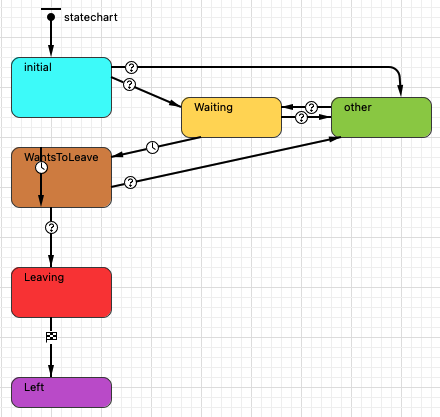
\includegraphics[width=300px]{patientStatechart}}   
    \caption{\textit{Statechart} dell'agente Patient}
    \label{fig:statechart}
\end{figure}

\subsection{Ambulance e AmbulancePatient}

Ambulance e AmbulancePatient sono le due classi di agenti definite per rappresentare i pazienti che giungono al pronto soccorso in ambulanza. Nell'ambiente hanno un'entrata prioritaria che permette loro di saltare le fasi di accettazione, triage e visita. 

Ambulance è definito ai fini del modello solo come mezzo di trasporto "contenitore" per i pazienti di tipo AmbulancePatient.
Viene generato uno di questi agenti all'occorrenza, ovvero quando un agente di tipo AmbulancePatient ha bisogno di essere trasportato in ambulanza fino al pronto soccorso. 

AmbulancePatient è un'estensione della classe che definisce l'agente Patient e mantiene dunque i suoi parametri descritti in precedenza; per questo agente viene però impostato di default il bisogno di un letto per la degenza, mentre gli altri parametri sono impostati come segue nel blocco di generazione: 
\begin{itemize}
    \item Priority: il valore viene generato da una distribuzione uniforme discreta con valori compresi tra 6 e 10. 
    \item Surgery: viene impostato un valore casuale tra yes e no. 
    \item Sickness: per gli arrivi in ambulanza viene sempre impostato a Red. 
\end{itemize}

\subsection{Nurse}
È l'agente che rappresenta gli infermieri: questi sono generati nel modello in un numero variabile in base all'impostazione del pool di risorse che li contiene. 
La classe che definisce l'agente non presenta parametri, funzioni o stati particolari ma serve a definire solo a livello estetico gli infermieri. 
Questi agenti sono utilizzati nel workflow del sistema esclusivamente tramite blocchi di tipo \textit{seize} e \textit{release}, che permettono di "riservarli" per un tempo utile ad eseguire una determinata azione (nel nostro caso, accompagnare i pazienti in varie stanze qualora ce ne sia bisogno). 

\section{Workflow}

Il workflow è la parte focale della costruzione del sistema tramite il software AnyLogic e viene mostrato interamente nella figura \ref{fig:wf-all}.
\\Permette infatti di far interagire agenti ed ambiente secondo determinate regole e condizioni, che possono essere specificate tramite la modellazione a blocchi e, per ciascun blocco, estese con linguaggio Java. 

In questa sezione verrà descritta ogni fase del workflow realizzato, al fine di far comprendere al lettore non solo il funzionamento del modello in sè, ma anche quali sono alcune delle funzionalità offerte da Anylogic. 

\begin{figure}[!htb]
    \centering
    \makebox[\textwidth][c]{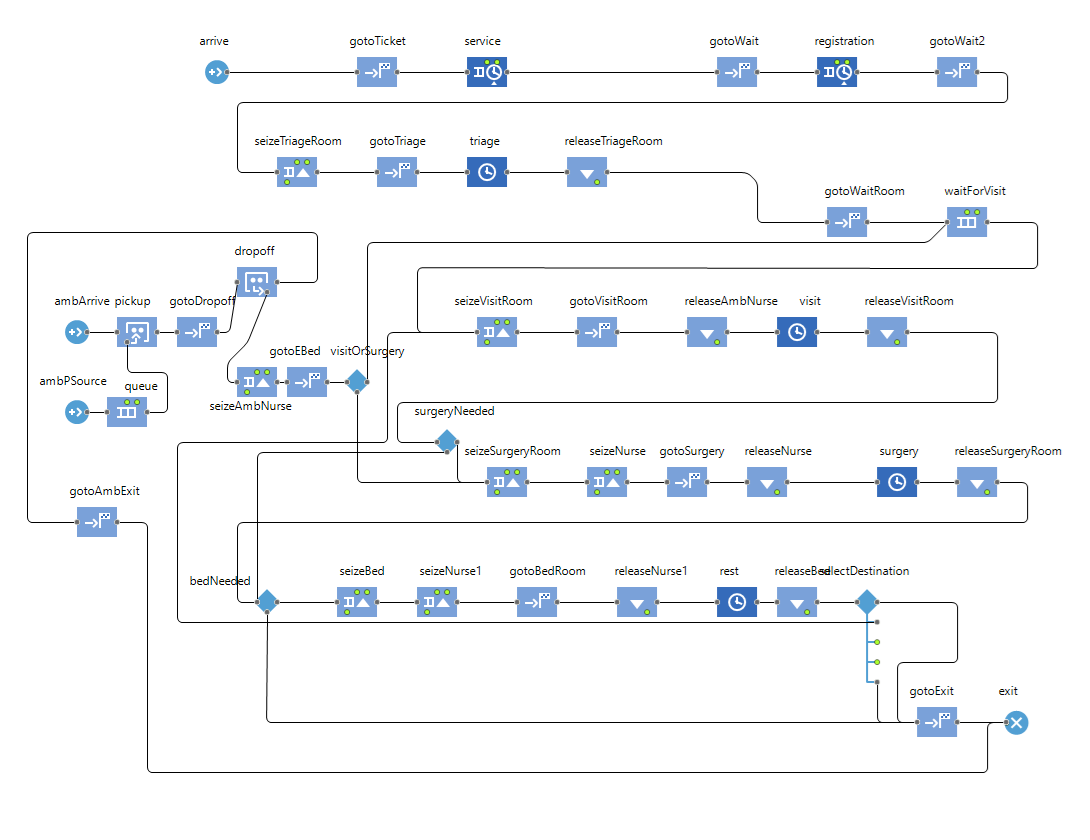
\includegraphics[width=1\textwidth]{workflow/wf-all}}   
    \caption{Workflow complessivo del sistema}
    \label{fig:wf-all}
\end{figure}

\clearpage
\subsection{Strumenti utilizzati nel Workflow} \label{chap:param}
Nell’implementazione della simulazione abbiamo avuto necesità di utilizzare degli strumenti, tra cui le \textit{resource pool} che ci hanno permesso di definire degli insiemi di unità che potevano essere riservate (\textit{seized}) e rilasciate (\textit{released}) dagli agenti che utilizzavano i seguenti tipi di blocco: \texttt{Seize}, \texttt{Release}, \texttt{Delay} e \texttt{Service}.

In particolare abbiamo definito i seguenti insiemi: infermieri, biglietteria, accettazione (Registrars), triage, sala visita, chirurgia e letti disponibili.

\begin{figure}[!htb]
    \centering
    \makebox[\textwidth][c]{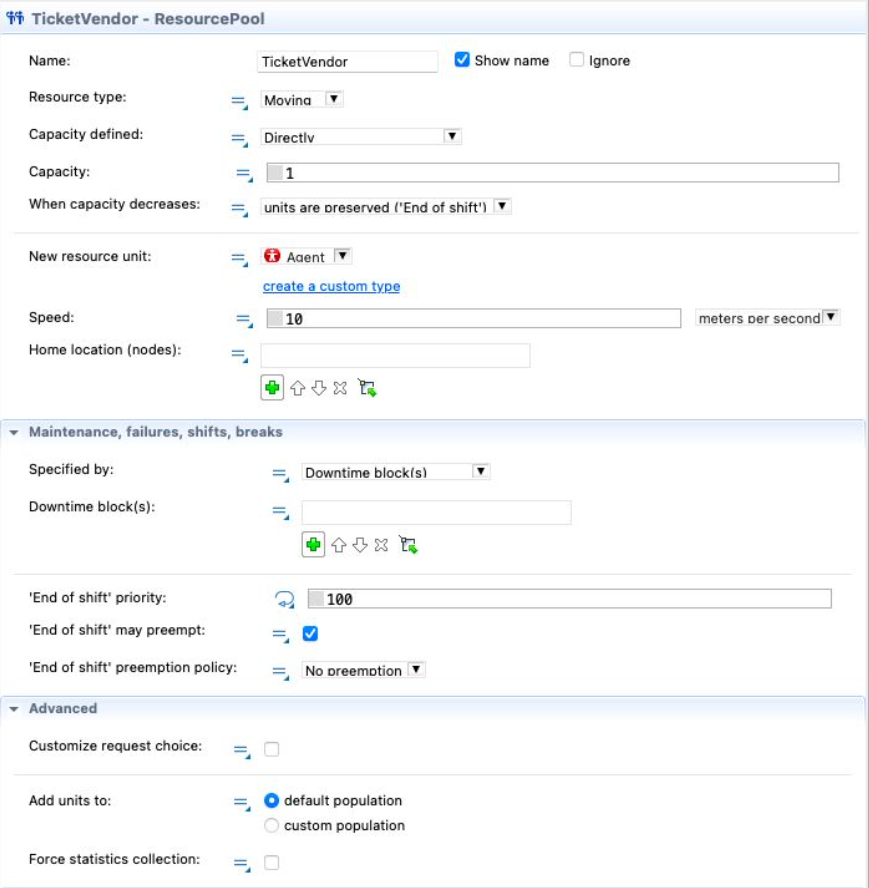
\includegraphics[width=350px]{Immagini/workflow/ResourcePool.png}}   
    \caption{Interfaccia Resource Pool}
\end{figure}

\clearpage
All'interno della simulazione è stato necessario inserire parametri e funzioni; i primi ci hanno permesso di definire delle caratteristiche statiche e le seconde sono state fondamentali per calcolare valori a runtime a seconda del percorso seguito dal paziente.  

All’interno del nostro \textit{Main} possiamo trovare tre funzioni e due parametri:
\begin{itemize}
\item \texttt{arrivalRate}: il numero di pazienti che arrivano per ora, che nel nostro caso è settato a 8 pazienti/ora.
\item \texttt{ambulanceArrRate}: il numero di pazienti che arrivano in ambulanza ogni ora (default 4 pazienti/ora). \\
\item \texttt{staffSpeed}: restituisce la velocità dello staff del pronto soccorso.
\item \texttt{patientSpeed}: restituisce  la velocità dei pazienti.
\item \texttt{restTime}: permette di calcolare il tempo che i pazienti necessitano di passare a letto, in base alla priorità assegnata.\\
\end{itemize}

\begin{figure}[!htb]
    \centering
    \makebox[\textwidth][c]{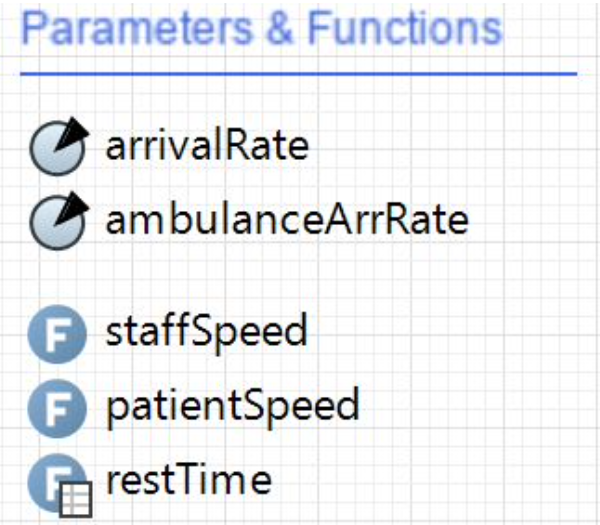
\includegraphics[width=200px]{Immagini/workflow/param.png}}   
    \caption{Parametri e Funzioni implementati}
\end{figure}
\clearpage
\subsection{L'arrivo del paziente}

Il nostro workflow ha due diversi punti d’inizio: il primo che andremo a trattare è il caso in cui il paziente arriva all'ospedale autonomamente, deve prendere il biglietto per poter sedersi in sala d’aspetto e successivamente essere chiamato per l’accettazione. Nel paragrafo \ref{chap:ambulance}  verrà trattato anche il caso in cui il paziente arrivi trasportato in ambulanza.

Questa parte del workflow comprende il blocco \texttt{arrive} da cui tutto il workflow ha inizio. All'interno di essp è possibile definire il rate di arrivo degli agenti (parametro \texttt{arrivalRate}) e la velocità che avranno nel modello (funzione \texttt{patientSpeed()}). 
Inoltre in questo blocco,  come in tutti quelli successivi, è possibile definire la zona della simulazione in cui avviene l’azione e quale agente specifico è coinvolto (Patient in questo caso). 

Il paziente arriva e va a prendere il biglietto con il blocco di movimento \texttt{gotoTicket} che segnala all’agente in che punto della simulazione recarsi.

Il blocco successivo \texttt{service} invece è quello designato per prendere il biglietto che sarà necessario per aspettare il turno dell’accettazione nella sala d’aspetto.\\ Questo blocco è particolare in quanto permette di prendere delle risorse da una \texttt{resource pool} (Ticket Machine), creare una coda di grandezza prestabilita e settare un delay: per entrambe le cose è possibile definire il nodo in cui le azioni devono avvenire. 

Dopo che l’agente ha preso il numero, con il blocco di movimento \texttt{gotoWait} si sposta in sala d’aspetto fino a che non verrà chiamato per effettuare l'accettazione.

\begin{figure}[!htb]
    \centering
    \makebox[\textwidth][c]{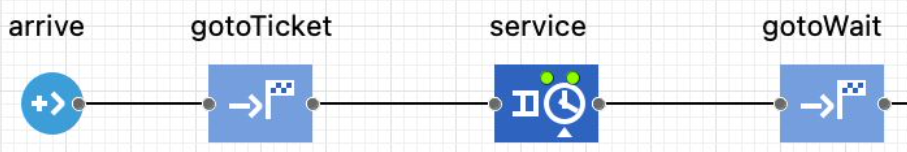
\includegraphics[width=1\textwidth]{Immagini/workflow/patient-arrive.png}}   
    \caption{Workflow dell'arrivo del paziente}
\end{figure}

\clearpage
\subsection{Triage}
L’agente entra nel blocco \texttt{registration} che preleva una persona, se libera, dalla resource pool \texttt{Registrars} che avrà il compito di fare l’accettazione al paziente (ne sono presenti due); inoltre è settato un delay secondo una distribuzione triangolare, che sarà il tempo impiegato per effettuare l’accettazione. \\ Infine, vengono delineate due zone: quella per aspettare in coda che l’accettazione sia libera e la zona in cui effettivamente effettuarla.\\ Dopo che il paziente effettua l’accettazione, tramite il blocco di movimento \texttt{gotoWait2} torna in sala d’aspetto.

Il blocco successivo \texttt{seizeTriageRoom} crea la coda di persone che nella \texttt{WaitingRoom} aspettano di venir chiamati per andare a fare il triage, richiede alla resource pool \texttt{TriageRooms} se ci sia una sala libera e nel caso ci fosse la riserva per il paziente; tramite il blocco \texttt{gotoTriage} l’agente ci si dirige, altrimenti rimane nella coda ad aspettare una sala libera.

Il triage viene eseguito dal blocco \texttt{triage} che ha la particolarità di creare un delay in cui verosimilmente viene effettuato un triage: da questo blocco il paziente uscirà con la diagnosi e gli verrà assegnata una priorità.

Alla fine di queste operazioni, tramite il blocco \texttt{release TriageRoom} 
viene liberata la sala per il triage 
che ritornerà disponibile nella resource pool \texttt{TriageRooms}.\\


\begin{figure}[!htb]
    \centering
    \makebox[\textwidth][c]{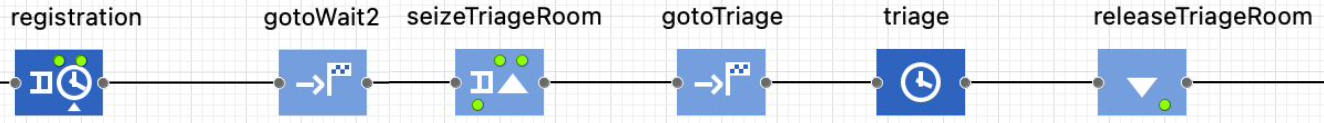
\includegraphics[width=1\textwidth]{Immagini/workflow/triage.png}}   
    \caption{Workflow del triage}
\end{figure}

\clearpage

\subsection{Visita Specialistica}
La priorità affidata al paziente sulla base della diagnosi sarà la discriminante per mandarlo direttamente alle sale visita (in casi di codice rosso) oppure ad aspettare in sala d’attesa.

Nel caso in cui il paziente non è troppo grave viene quindi mandato nella sala d’attesa (\texttt{gotoWaitRoom}) e si mette in fila (\texttt{wairForVisit}), quest'ultima gestita secondo una politica priority-based (a seconda della priorità di ciascun paziente).

Quando il paziente è il primo della coda, viene controllato se nella resource pool \texttt{VisitRooms} vi sia una sala visita libera e nel caso vi sia viene mandato a fare la visita (\texttt{gotoVisitRoom}).
 
Durante la visita viene valutato se sia necessaria la chirurgia e/o un letto. Al termine della visita viene 
rilasciata la sala visita (\texttt{releaseVisitRoom}) che torna nella resource pool \texttt{VisitRooms}. \\


\begin{figure}[!htb]
    \centering
    \makebox[\textwidth][c]{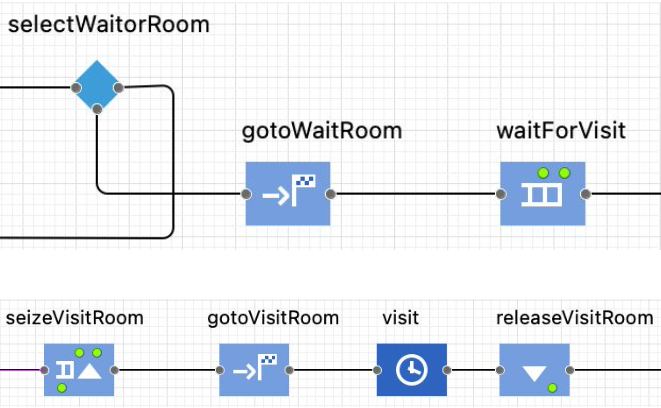
\includegraphics[width=250px]{Immagini/workflow/visit.png}}   
    \caption{Workflow di una visita specialistica}
\end{figure}

\clearpage
\subsection{Chirurgia}  
Nel caso in cui il paziente avesse bisogno di un intervento in chirurgia (\texttt{surgeryNeeded}) viene verificato che ci siano delle sale operatorie (\texttt{seize SurgeryRoom}) e 
infermieri (\texttt{seizeNurse}) liberi.
\\ Se queste due condizioni sono verificare il paziente viene spostato in chirurgia con l'aiuto dell’infermiere (\texttt{gotoSurgery}) che viene rilasciato (\texttt{releaseNurse}) nel momento in cui il paziente arriva nella sala, tornando al nodo \texttt{staffRoom}. \\
L’intervento (\texttt{surgery}) dura per un tempo variabile che segue una distribuzione triangolare e nel momento in cui finisce la sala viene liberata (\texttt{release SurgeryRoom}).


\begin{figure}[!htb]
    \centering
    \makebox[\textwidth][c]{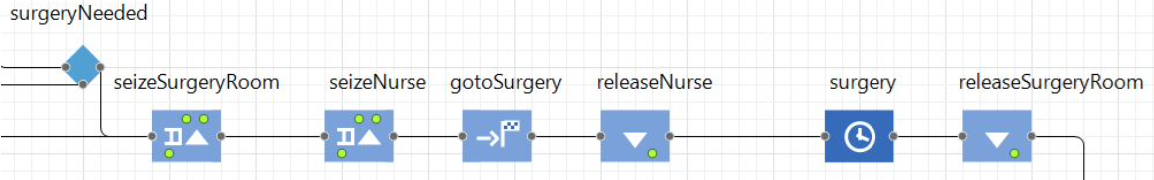
\includegraphics[width=1\textwidth]{Immagini/workflow/chirurgia.png}}   
    \caption{Workflow di un intervento chirurgico}
\end{figure}

\subsection{Degenza e uscita}  
Il paziente può aver bisogno di un letto in due casi: se ha avuto un intervento chirurgico oppure ha bisogno di essere genericamente monitorato. 

Viene quindi controllato che ci siano un letto disponibile (\texttt{seizeBed}) e un infermiere libero (\texttt{seizeNurse1}) per accompagnare il paziente nella degenza (\texttt{gotoBedRoom}), infermiere che torna a disposizione dopo aver portato il paziente (\texttt{releaseNurse1}).

Durante la degenza (\texttt{rest}) i pazienti possono aver bisogno di ulteriori visite (seconda uscita del blocco \texttt{selectDestination}) oppure i problemi possono risolversi ed essere dimessi (prima e ultima uscita, ovvero quella di default). Dopo un delay variabile a seconda della gravità del paziente questo parametro viene aggiornato.

Nel caso in cui non fosse necessaria un’ulteriore visita il paziente può uscire (\texttt{gotoExit}) liberando il letto (\texttt{releaseBed}).


\begin{figure}[!htb]
    \centering
    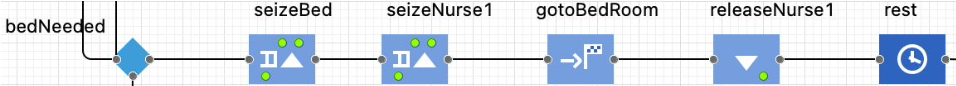
\includegraphics[width=1\textwidth]{Immagini/workflow/bed1.png}
\end{figure}
\begin{figure}[!htb]
    \centering
    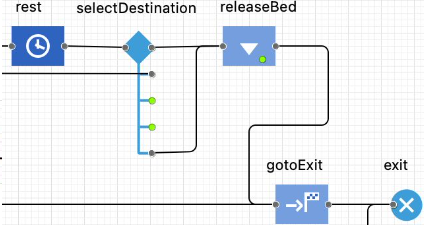
\includegraphics[width=220px]{Immagini/workflow/bed2.png} 
    \caption{Workflow della degenza e dll'uscita}
\end{figure}

\subsection{Arrivo in Ambulanza} \label{chap:ambulance}

Un paziente oltre a poter arrivare al pronto soccorso da solo può arrivare in ambulanza.

Le ambulanze vengono generate dal blocco \texttt{ambArrive} ogni qualvolta un paziente ha bisogno del loro intervento.

I pazienti bisognosi vengono creati dal blocco \texttt{ambPSource}, dal quale poi vengono inviati in una coda per attendere l’arrivo dell’ambulanza. All’entrata nel blocco di coda, viene invocata la funzione \texttt{inject()} sul blocco di generazione delle ambulanze per chiamarne una all’occorrenza. 

L’ambulanza funge da container e  tramite il blocco \texttt{pickup} carica il paziente e lo scarica (tramite \texttt{dropoff}) all’entrata per ambulanze del pronto soccorso, dove gli viene riservato un infermiere per portarlo ad effettuare una visita o, nei casi più urgenti, una chirurgia.

\begin{figure}[!h]
    \centering
    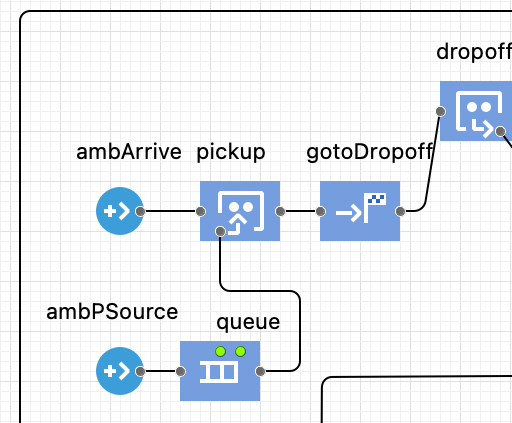
\includegraphics[width=250px]{Immagini/workflow/Ambulance.png} 
    \caption{Workflow dell'arrivo in ambulanza}
\end{figure}




\chapter{Sperimentazioni e Risultati} \label{chap:sper}
Le potenzialità di AnyLogic ci permettono di fare varie sperimentazioni sul modello
che abbiamo costruito. In particolare ci andremo a concentrare sulla distribuzione 
della gravità dei pazienti, basandoci sui codici con cui arrivano al pronto soccorso, per valutare la risposta della nostra simulazione.

Valuteremo i seguenti casi:
\begin{itemize}
    \item \textbf{Distribuzione Uniforme}: utilizziamo il random su option list fornita da AnyLogic.
    \item \textbf{Distribuzione Personalizzata}: utilizziamo la nostra distribuzione personalizzata in cui i codici si presentano con le seguenti percentuali:
    \begin{itemize}
        \item $25\%$ codici bianchi
        \item $40\%$ codici verdi
        \item $25\%$ codici gialli
        \item $10\%$ codici rossi
    \end{itemize}
\end{itemize}

\clearpage
Inoltre, avendo la possibilità di personalizzare i parametri dei nostri agenti è stato possibile:
\begin{itemize}
    \item  \texttt{appearence = uniform${\_}$discr(1, 3)}: dare un indicazione di come avremo voluto che apparissero
    \item \texttt{priority = 0} e \texttt{surgery = no}: il livello di priorità iniziale e la necessità di intervento che vengono impostati a zero e successivamente modificati durante il blocco di \texttt{triage}.
    \item \texttt{bed = yesB}: si pensa che le persone arrivino genericamente con una condizione che necessiterà di una breve degenza (anche di minuti), anche questo può venir modificato durante il workflow.
    \item \texttt{initial speed = 5}: la velocità iniziale del paziente che è stata impostata a $5$km all'ora in accordo con i risultati medi dei paper consultati.
\end{itemize}

All'interno del \textit{Main} della simulazione sono presenti anche delle funzioni e parametri che sono stati precedentemente presentati nel capitolo \ref{chap:param} che abbiamo impostato con i seguenti valori:

\begin{itemize}
    \item \texttt{arrivalRate = 8}: le persone che arrivano in ospedale autonomamente sono 8 all'ora.
    \item \texttt{ambulanceArrRate = 4}: il numero di ambulanze che arrivano in ospedale sono 4 all'ora.
    \item \texttt{staffSpeed()}: ritorna una distribuzione uniforme \texttt{uniform(3.3, 4.2)}.
    \item \texttt{patientSpeed()} ritorna una distribuzione uniforme \texttt{uniform(2.5, 3.5)}.
    \item \texttt{restTime()}: è una funzione costruita per simulare il tempo necessario nella degenza per un paziente, è modellata come in figura \ref{fig:function}.
\end{itemize}
\clearpage

\begin{figure}[!h]
    \centering
    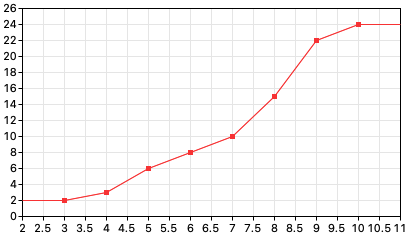
\includegraphics[width=300px ]{Immagini/function.png} 
    \caption{restTime()}
    \label{fig:function}
\end{figure}


Le \textit{resource pool} hanno anch'esse dei valori che possono essere impostati e nel nostro modello ci siamo soffermati in particolare sul numero di elementi che componevano ogni pool che riportiamo:
\begin{itemize}
\item \texttt{Nurses = 10}
\item \texttt{Registrars = 2}
\item \texttt{TriageRooms = 2}: viene impostata in base alle stanze per il triage effettivamente esistenti, nel nostro caso due.
\item \texttt{TicketMachine = 1}
\item \texttt{VisitRooms = 4}: viene impostata in base alle sale visita effettivamente esistenti, nel nostro caso quattro.
\item \texttt{SurgeryRooms = 2}: viene impostata in base alle sale operatorie effettivamente esistenti, nel nostro caso due.
\item \texttt{Beds = 10}
\end{itemize}

\section{Sperimentazioni e Parametri utilizzati} \label{par:esp}

Per poter analizzare propriamente le conseguenze del cambiamento delle variabili sopra descritte, abbiamo definito alcune statistiche che ci permettessero di visualizzare alcune delle metriche più importanti:

\begin{itemize}
    \item \textit{Tempo totale di permanenza, per paziente (minuti)}
    \item \textit{Numero di pazienti presenti nel pronto soccorso, nel tempo}
    \item \textit{Tempo di attesa medio (minuti)}
\end{itemize}

I risultati ottenuti sono stati successivamente confrontati con quelli ottenuti dagli autori dei lavori precedenti (\textit{\cite{espinoza_real-time_2014}}).

Tutte le sperimentazioni sono state eseguite per 500 minuti.

\subsection{Prima sperimentazione} 
I valori dei parametri, per questo primo tentativo, sono stati mantenuti come descritti nei paragrafi precedenti, ovvero arrivano 8 pazienti e 4 ambulanze all'ora. 
Questa sperimentazione sarà utilizzata nel seguito come "caso di default" per i confronti.


Quello che possiamo vedere dall'osservazione di questa iterazione sono i seguenti valori medi riportati in figura \ref{fig:graf1} anche sotto riportati:
\begin{itemize}
    \item \textit{Tempo medio di permanenza:} 163 minuti.
    \item \textit{Numero di pazienti presenti nel pronto soccorso, nel tempo}: 54 pazienti.
    \item \textit{Tempo di attesa medio:} 91 minuti.
\end{itemize}


Possiamo vedere che il numero di pazienti andrebbe ad aumentare così come il tempo medio, e questo potrebbe portare ad una saturazione del pronto soccorso.

\begin{figure}[!h]
    \centering
    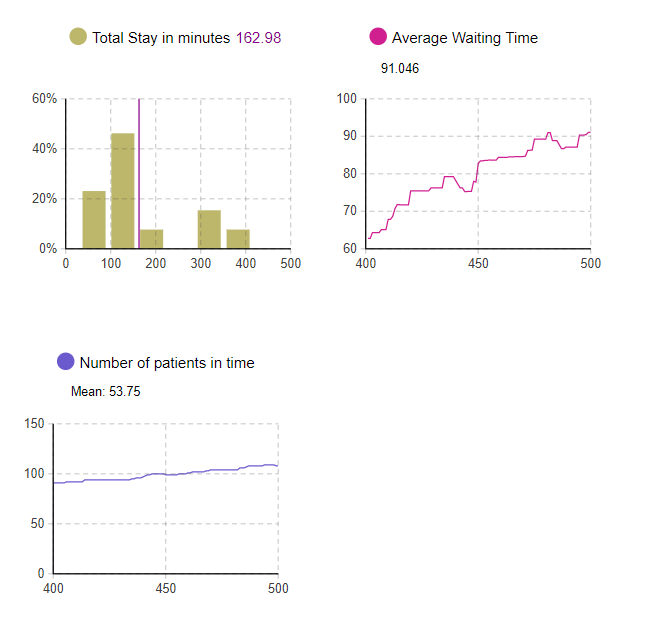
\includegraphics[width=1\textwidth]{Immagini/sper1.png} 
    \caption{Grafici delle metriche della prima sperimentazione}
    \label{fig:graf1}
\end{figure}
\clearpage
\subsection{Seconda Sperimentazione} \label{cahp:seconda}
I valori dei parametri, in questa seconda configurazione, sono stati raddoppiati rispetto alla prima sperimentazione, ovvero arrivano 16 pazienti e 8 ambulanze all'ora. 


Per questa sperimentazione troviamo come valori delle metriche:
\begin{itemize}
    \item \textit{Tempo medio di permanenza:} 221 minuti.
    \item \textit{Numero di pazienti presenti nel pronto soccorso, nel tempo}: 84 pazienti.
    \item \textit{Tempo di attesa medio:} 98 minuti.
\end{itemize}

\subsection{Terza Sperimentazione}
Per eseguire il terzo esperimento abbiamo mantenuto i valori di default per quanto riguarda il tasso di arrivo di ambulanze e pazienti (8 pazienti/ora, 4 ambulanze/ora), modificando però la distribuzione del parametro \textit{sickness} (dei pazienti arrivati a piedi) con una distribuzione uniforme, invece che basarla su percentuali più realistiche come impostato in precedenza. 

Con questa configurazione i risultati ottenuti sono i seguenti: 
\begin{itemize}
    \item \textit{Tempo medio di permanenza:} 143 minuti.
    \item \textit{Numero di pazienti presenti nel pronto soccorso, nel tempo}: 46 pazienti.
    \item \textit{Tempo di attesa medio:} 78 minuti.
\end{itemize}


\subsection{Quarta Sperimentazione}
Per l'esecuzione del quarto esperimento abbiamo scelto di modificare il tempo di attesa nel triage abbassandolo (\texttt{triangular(2, 20, 5)} $\rightarrow$ \texttt{triangular(2, 10, 5)}) e riportare le percentuali di \textit{sickness} su una distribuzione realistica ed abbiamo ottenuto i seguenti risultati.

\begin{itemize}
    \item \textit{Tempo medio di permanenza:} 156 minuti.
    \item \textit{Numero di pazienti presenti nel pronto soccorso, nel tempo}: 53 pazienti.
    \item \textit{Tempo di attesa medio:} 76 minuti.
\end{itemize}

\subsection{Quinta Sperimentazione}
L'ultima sperimentazione effettuata ha previsto l'aumento del numero di infermieri disponibili, da 10 a 20, mantenendo i tassi di arrivo di default. 

I risultati ottenuti sono i seguenti: 
\begin{itemize}
    \item \textit{Tempo medio di permanenza:} 142 minuti.
    \item \textit{Numero di pazienti presenti nel pronto soccorso, nel tempo}: 53 pazienti.
    \item \textit{Tempo di attesa medio:} 89 minuti.
\end{itemize}

\section{Risultati}

In seguito alle sperimentazioni effettuate con i parametri impostati come precedentemente presentato nel paragrafo \ref{par:esp}, abbiamo potuto osservare e trarre le seguenti conclusioni: 

\begin{enumerate}
    \item A parità di tasso di arrivo, una distribuzione uniforme dei codici dei pazienti (per quanto irrealistica) migliora di molto l'efficienza in tutte e tre le metriche analizzate, come prevedibile. Tuttavia non si avrà mai questo caso nella realtà;
    \item La diminuzione del tempo massimo di triage ha un leggero impatto sul tempo di attesa medio, che passa da 91 minuti del caso di default a 76 minuti;
    \item Il raddoppio dei tassi di arrivo adottato nella seconda sperimentazione influisce negativamente in maniera sostanziale sul tempo medio di permanenza, mentre non impatta troppo il tempo di attesa medio;
    \item L'aumento del numero di infermieri disponibili non migliora quasi per nulla l'efficienza rispetto al caso di default. Questo può essere dovuto al fatto che gli infermieri, nel nostro modello, hanno mansioni di solo accompagnamento che difficilmente portano ad una saturazione delle risorse disponibili.  
\end{enumerate}

In conclusione, da quanto osservato, possiamo dire che per aumentare il più possibile l'efficienza del modello e di conseguenza quella di un caso reale, non essendo evidentemente possibile diminuire sempre il tempo massimo di visite e triage o prevedere una distribuzione uniforme della gravità dei pazienti, si potrebbe pensare di aumentare la capacità del pronto soccorso con nuove stanze, permettendo così il trattamento di più pazienti in parallelo. 

È tuttavia da sottolineare che nel presente modello non sono state considerate varie problematiche reali come ad esempio il cambio di turno dello staff o la sua non-disponibilità, che potrebbero peggiorare di molto le metriche prese in considerazione. 

\section{Confronto con lavori precedenti}

I risultati ottenuti nei paper di riferimento per la costruzione del modello non sono perfettamente comparabili con i risultati da noi osservati poiché essi utilizzavano varie distinzioni di scenari maggiormente complessi ed articolati rispetto al nostro lavoro.

Possiamo però sottolineare come in \textit{\cite{espinoza_real-time_2014}} vengano messi in evidenza il numero di accessi al pronto soccorso durante il giorno al variare del giorno della settimana considerato. Valutando una media degli accessi giornalieri possiamo vedere una media che si mantiene tra i 6 e gli 8 pazienti all'ora, con picchi fino a 12 nelle ore più congestionare e 2 nelle ore notturne. Nella nostra simulazione abbiamo provato a simulare un momento di particolare congestione nel paragrafo \ref{cahp:seconda} arrivando a sedici pazienti e quattro ambulanze all'ora. Da notare però che il tempo medio di attesa in tutte queste condizione rimane sostanzialmente inferiore a quello dai noi osservato (dai 10 ai 37 minuti rispetto ai 76-98 del nostro modello).
In merito però a questi risultati possiamo però dire che la simulazione presentata nel paper ha delle differenze sostanziali nella costruzione del pronto soccorso basandosi su una struttura esistente ed i tempi non derivano da una simulazione ma dall'osservazione reale del fenomeno.

Per questo motivo, se pure si è cercato di imitare un contesto realistico e vicino alla realtà, abbiamo comunque scelto di generalizzare piuttosto che andare nello specifico di un singolo pronto soccorso esistente e per questo motivo i dati dei paper non coincidono perfettamente con i nostri.

\chapter{Conclusioni}

In conclusione, date le osservazioni ricavate dalle sperimentazioni effettuate possiamo affermare che il software AnyLogic si dimostra uno strumento utile per supportare la simulazione di scenari che hanno bisogno di essere ottimizzati, valutarne possibili estensioni o semplicemente per rispondere a domande del tipo \textit{“what if…?”}.


La palette di tool disponibili, dalla libreria per la modellazione del movimento di pedoni a quella per la modellazione del movimento di fluidi, lo rende uno strumento versatile ed utilizzabile in moltissimi ambiti. 

La modellazione a blocchi rende questo strumento easy to learn, ma le molte funzionalità e il fatto di essere basato completamente su Java lo rendono hard to master; inoltre la possibilità di integrare algoritmi di learning è interessante, ma non è compresa direttamente nel software sebbene con \textit{Pathmind} sia possibile avere un Helper integrato. 

Nel caso della nostra simulazione è risultato difficile integrare algoritmi di learning: gli agenti che abbiamo modellato seguivano un workflow preciso ed ognuno di essi non perseguiva un obiettivo, ma si muoveva in base al prossimo blocco presente nel flusso. 

Bisogna menzionare che è sempre tuttavia possibile osservare o modificare le variabili a runtime, tramite controlli, per vedere come reagisce il modello. Questo ci permette di avere un controllo maggiore sulla simulazione e di poter effettuare anche degli \textit{“stress test”}.
Molto interessante anche la possibilità di inserire statistiche per le popolazioni di agenti ed osservarne l’andamento tramite grafici, per una miglior comprensione dell'andamento. 

AnyLogic è uno strumento molto ampio e sarebbe necessaria una quantità di tempo più elevata per realizzare e simulare modelli più complessi, ma ciò nonostante si è  presentato pratico e funzionale per la realizzazione del modello scelto.
\printbibliography

\end{document}